%\begin{enumerate}[1.]
%\numberwithin{equation}{\thesubsection.enumi}

%\begin{enumerate}[label=\arabic*.,ref=\thesection]
\renewcommand{\theequation}{\theenumi}
\begin{enumerate}[label=\arabic*.,ref=\thesubsection.\theenumi]
%\begin{enumerate}[label=\arabic*.,ref=\thesubsection.\theenumi]
%\numberwithin{equation}{subsection}

%\begin{enumerate}[label=\arabic*.,ref=\thesubsection.\theenumi]
%\begin{enumerate}[label=\thesection.\arabic*,ref=\thesection.\theenumi]

%\numberwithin{equation}{enumi}
\item Find the distance between 
\begin{align}
\vec{P} = \myvec{-2\\4}, \vec{Q} = \myvec{3\\-5}
\end{align}
%Mark on a diagram the points $\myvec{-2,4}, \myvec{3,-5}$ and find the distance between them.
\solution
The general second order equation can be expressed as follows,
\begin{align}
\vec{x^T}\vec{V}\vec{x}+2\vec{u^T}\vec{x}+f=0\label{eq:solutions/3/4/11/eq:1}
\end{align}
Comparing \eqref{eq:solutions/3/4/11/eq:0} with \eqref{eq:solutions/3/4/11/eq:1},
\begin{align}
\vec{V} = \myvec{5 & 1\\1 & 5}\label{eq:solutions/3/4/11/eq:2}\\
\vec{u} = \myvec{-7\\ -11}\label{eq:solutions/3/4/11/eq:3}\\
f = 27\label{eq:solutions/3/4/11/eq:4}
\end{align}
Let $\vec{c}$ be the change in the origin. The equation \eqref{eq:solutions/3/4/11/eq:1} can be modified as
\begin{align}
\vec{(x+c)^T}\vec{V}\vec{(x+c)}+2\vec{u^T}\vec{(x+c)}+f=0\label{eq:solutions/3/4/11/eq:5}
\end{align}
Considering \eqref{eq:solutions/3/4/11/eq:5}
\begin{align}
&\implies \vec{(x+c)^T}\vec{V}\vec{(x+c)}\\
&\implies \vec{x^T}\vec{V}\vec{x}+\vec{c^T}\vec{V}\vec{x}+\vec{x^T}\vec{V}\vec{c}+\vec{c^T}\vec{V}\vec{c}\label{eq:solutions/3/4/11/eq:6}
\end{align}
In the above equation
\begin{align}
\vec{c^T}\vec{V}\vec{x} = \vec{x^T}\vec{V}\vec{c}\label{eq:solutions/3/4/11/eq:7}
\end{align}
From \eqref{eq:solutions/3/4/11/eq:6} and \eqref{eq:solutions/3/4/11/eq:7} then \eqref{eq:solutions/3/4/11/eq:5} becomes
\begin{align}
\vec{x^T}\vec{V}\vec{x}+2\vec{c^T}\vec{V}\vec{x}+\vec{c^T}\vec{V}\vec{c}+2\vec{u^T}\vec{x}+2\vec{u^T}\vec{c}+f = 0\label{eq:solutions/3/4/11/eq:8}
\end{align}
Comparing \eqref{eq:solutions/3/4/11/eq:0.1} and \eqref{eq:solutions/3/4/11/eq:8}
\begin{align}
2\vec{c^T}\vec{V}\vec{P}\vec{y} + 2\vec{u^T}\vec{P}\vec{y} =0\\
\vec{c^T}\vec{V}\vec{P}\vec{y} = - \vec{u^T}\vec{P}\vec{y}\\
\vec{c} = -\vec{V^{-1}}\vec{u}\label{eq:solutions/3/4/11/eq:9}
\end{align}
Substituting \eqref{eq:solutions/3/4/11/eq:2} and \eqref{eq:solutions/3/4/11/eq:3} in \eqref{eq:solutions/3/4/11/eq:9}
\begin{align}
\vec{c}=\frac{-1}{24}\myvec{5&-1\\-1&5}\myvec{-7\\-11}=\myvec{1\\2 }\label{eq:solutions/3/4/11/eq:10}
\end{align}
Hence \eqref{eq:solutions/3/4/11/eq:8} becomes
\begin{align}
\vec{x^T}\vec{V}\vec{x}+\vec{c^T}\vec{V}\vec{c}+2\vec{u^T}\vec{c}+f = 0 \label{eq:solutions/3/4/11/eq:11}
\end{align}
Substituting \eqref{eq:solutions/3/4/11/eq:2}, \eqref{eq:solutions/3/4/11/eq:3} and \eqref{eq:solutions/3/4/11/eq:10} the above equation becomes
\begin{align}
\vec{x^T}\myvec{5&1\\1&5}\vec{x}+\myvec{1&2}\myvec{5&1\\1&5}\myvec{1\\2}+2\myvec{-7&-11}\myvec{1\\2}\\+27 = 0
\end{align}
\begin{align}
\vec{x^T}\myvec{5&1\\1&5}\vec{x}+29-58+27=0\\
\vec{x^T}\vec{V}\vec{x}-2 = 0\label{eq:solutions/3/4/11/eq:12}
\end{align}
With change in the origin to point $\vec{c}=\myvec{1\\2}$ but the $\vec{V}$ doesn't change.
\begin{align}
\mydet{\vec{V}} = \mydet{5&1\\1&5} = 24
\end{align}
As $\mydet{\vec{V}} >0$ it represents a ellipse.Hence $\vec{V}$ can be written as,
\begin{align}
\vec{V}=\vec{P}\vec{D}\vec{P^T}\label{eq:solutions/3/4/11/eq:13}
\end{align}
 The characteristic equation of $\vec{V}$ is given by
\begin{align}
\mydet{\vec{V}-\vec{I}\lambda} = 0\\
\mydet{5-\lambda & 1\\1& 5-\lambda} =0\\
\implies \lambda^2 - 10\lambda+24 = 0
\end{align}
Hence the eigen vales are,
\begin{align}
\lambda_1 = 4\\
\lambda_2 = 6
\end{align}
Hence diagonal vector is given by,
\begin{align}
\vec{D}= \myvec{\lambda_1&0\\0&\lambda_2} = \myvec{4&0\\0&6}\label{eq:solutions/3/4/11/eq:14}
\end{align}
The eigen vector $\vec{p}$ is given by
\begin{align}
    \vec{V}\vec{p}&=\lambda\vec{p}\\
    (\vec{V}-\lambda\vec{I})\vec{p}&=0
\end{align}
For $\lambda_1 = 4$  the eigenvector is,
\begin{align}
\vec{V}-\lambda_1\vec{I}= \myvec{1&1\\1&1} \xleftrightarrow[]{R_2 \leftarrow R_2-R_1}\myvec{1&1\\0&0}\\
\vec{p_1}=\myvec{\frac{1}{\sqrt{2}}\\\frac{-1}{\sqrt{2}}}
\end{align}
For $\lambda_1 = 6$  the eigenvector is,
\begin{align}
\vec{V}-\lambda_1\vec{I}= \myvec{-1&1\\1&-1} \xleftrightarrow[]{R_2 \leftarrow R_2+R_1}\myvec{-1&1\\0&0}\\
\vec{p_1}=\myvec{\frac{1}{\sqrt{2}}\\\frac{1}{\sqrt{2}}}
\end{align}
Hence,
\begin{align}
\vec{P} =\myvec{\vec{p_1}&\vec{p_2}} = \myvec{\frac{1}{\sqrt{2}}&\frac{1}{\sqrt{2}}\\\frac{-1}{\sqrt{2}}&\frac{1}{\sqrt{2}}} \label{eq:solutions/3/4/11/eq:15}
\end{align}
Substituting \eqref{eq:solutions/3/4/11/eq:14} and \eqref{eq:solutions/3/4/11/eq:15} in \eqref{eq:solutions/3/4/11/eq:13}
\begin{align}
\vec{V}= \myvec{\frac{1}{\sqrt{2}}&\frac{1}{\sqrt{2}}\\\frac{-1}{\sqrt{2}}&\frac{1}{\sqrt{2}}}\myvec{4&0\\0&6}\myvec{\frac{1}{\sqrt{2}}&\frac{-1}{\sqrt{2}}\\\frac{1}{\sqrt{2}}&\frac{1}{\sqrt{2}}}\label{eq:solutions/3/4/11/eq:16}
\end{align}
Hence substituting \eqref{eq:solutions/3/4/11/eq:16} in \eqref{eq:solutions/3/4/11/eq:12}
\begin{align}
\vec{x^T}\myvec{\frac{1}{\sqrt{2}}&\frac{1}{\sqrt{2}}\\\frac{-1}{\sqrt{2}}&\frac{1}{\sqrt{2}}}\myvec{4&0\\0&6}\myvec{\frac{1}{\sqrt{2}}&\frac{-1}{\sqrt{2}}\\\frac{1}{\sqrt{2}}&\frac{1}{\sqrt{2}}}\vec{x}=2\\
\vec{y^T}\myvec{4&0\\0&6}\vec{y}=2\\
\vec{y^T}\myvec{2&0\\0&3}\vec{y}=1\label{eq:solutions/3/4/11/eq:17}
\end{align}
where $\vec{y}$ is given by Affine transformation
\begin{align}
\vec{x}=\vec{P}\vec{y} \\
\vec{y}=\vec{P^T}\vec{x} \label{eq:solutions/3/4/11/eq:22}
\end{align}
The rotation matrix $\vec{P}$ can be given by,
\begin{align}
\vec{P}=\myvec{\cos{\theta}&\sin{\theta}\\-\sin{\theta}&\cos{\theta}}\label{eq:solutions/3/4/11/eq:18}
\end{align}
Comparing \eqref{eq:solutions/3/4/11/eq:15} and \eqref{eq:solutions/3/4/11/eq:18}
\begin{align}
\cos{\theta} = \frac{1}{\sqrt{2}}\\
\theta = \frac{\pi}{4} 
\end{align}
But given the direction of coordinate axes changes so,
\begin{align}
\theta = \pi +\frac{\pi}{4}\label{eq:solutions/3/4/11/eq:19}
\end{align}
Subtituting \eqref{eq:solutions/3/4/11/eq:19} in \eqref{eq:solutions/3/4/11/eq:18} we get 
\begin{align}
\vec{P}=\myvec{\cos{\brak{\pi +\frac{\pi}{4}}} & \sin{\brak{\pi +\frac{\pi}{4}}}\\-\sin{\brak{\pi +\frac{\pi}{4}}}&\cos{\brak{\pi +\frac{\pi}{4}}}}\\
\vec{P}=\myvec{\frac{-1}{\sqrt{2}}&\frac{-1}{\sqrt{2}}\\\frac{1}{\sqrt{2}}&\frac{-1}{\sqrt{2}}}\label{eq:solutions/3/4/11/eq:20}
\end{align}
From \eqref{eq:solutions/3/4/11/eq:13} we find the diagonal matrix
\begin{align}
\vec{D}=\vec{P^T}\vec{V}\vec{P} = \myvec{\frac{-1}{\sqrt{2}}&\frac{1}{\sqrt{2}}\\\frac{-1}{\sqrt{2}}&\frac{-1}{\sqrt{2}}}\myvec{5&1\\1&5}\myvec{\frac{-1}{\sqrt{2}}&\frac{-1}{\sqrt{2}}\\\frac{1}{\sqrt{2}}&\frac{-1}{\sqrt{2}}}\\
\vec{D}=\myvec{6&0\\0&4}\label{eq:solutions/3/4/11/eq:21}
\end{align}
Hence using \eqref{eq:solutions/3/4/11/eq:20}, \eqref{eq:solutions/3/4/11/eq:21} and \eqref{eq:solutions/3/4/11/eq:13} in \eqref{eq:solutions/3/4/11/eq:12} we get.
\begin{align}
\vec{x^T}\myvec{\frac{-1}{\sqrt{2}}&\frac{-1}{\sqrt{2}}\\\frac{1}{\sqrt{2}}&\frac{-1}{\sqrt{2}}}\myvec{6&0\\0&4}\myvec{\frac{-1}{\sqrt{2}}&\frac{1}{\sqrt{2}}\\\frac{-1}{\sqrt{2}}&\frac{-1}{\sqrt{2}}}\vec{x}=2
\end{align}
using \eqref{eq:solutions/3/4/11/eq:22} the above equation becomes,
\begin{align}
\vec{y^T}\myvec{6&0\\0&4}\vec{y}=2\\
\vec{y^T}\myvec{3&0\\0&2}\vec{y}=1\label{eq:solutions/3/4/11/eq:23}
\end{align} 
Hence from \eqref{eq:solutions/3/4/11/eq:17} and \eqref{eq:solutions/3/4/11/eq:23} proved that change of origin and the directions of the coordinate axes \eqref{eq:solutions/3/4/11/eq:0} can be tranformed to \eqref{eq:solutions/3/4/11/eq:0.1} or \eqref{eq:solutions/3/4/11/eq:0.2}
\begin{figure}[!ht]
\centering
\includegraphics[width=\columnwidth]{./solutions/3/4/11/Ellipse.png}
\caption{Ellipse}
\label{eq:solutions/3/4/11/fig:Ellipse}
\end{figure}


%
\item
Find the length of $PQ$ for
\begin{enumerate}
\item $\vec{P}=\myvec{-1\\1}$ and $\vec{Q}=\myvec{2\\-1}$;
\item $\vec{P}=\myvec{4\\3}$ and $\vec{Q}=\myvec{-2\\2}$;
\item $\vec{P}=\myvec{a\\b}$ and $\vec{Q}=\myvec{-b\\a}$.
\end{enumerate}

\item Using direction vectors, show that  $\myvec{2\\1}, \myvec{4\\7}, \myvec{5\\4}$ and $\myvec{1\\4}$ are the vertices of a parallelogram.
\item Using Baudhayana's theorem, show that the points $\myvec{-3\\-4}, \myvec{2\\6}$ and $\myvec{-6\\10}$  are the vertices of a right-angled
traingle.  Repeat using orthogonality.
\item Plot the points $\myvec{0\\2},\myvec{1\\1},\myvec{4\\4}\text{ and }\myvec{3\\5}$ and prove that they are the vertices of a rectangle.
\item Show that $\vec{B}=\myvec{-2\\-2},\vec{A}=\myvec{-1\\2}\text{ and }\vec{C}=\myvec{3\\1}$ are the vertices of an isosceles triangle.
\item In the last question, find the distance of the vertex $\vec{A}$ of the triangle from the middle point of the base $BC$.
\item Prove that the points $\myvec{-1\\0}$, $\myvec{0\\3}$, $\myvec{3\\2}$ and $\myvec{2\\-1}$ are the vertices of a square.
\item Prove that the points $\vec{A}=\myvec{-1\\0}$, $\vec{B}=\myvec{3\\1}$, $\vec{C}=\myvec{2\\2}$  and $\vec{D}=\myvec{-2\\1}$ are the vertices of a parallelogram.  Find $\vec{E},\vec{F},\vec{G},\vec{H}$, the mid points of $AB, BC, CD, AD$ respectively.  Show that EG and FH bisect each other.
\item Prove that the points $\myvec{21\\-2}$, $\myvec{15\\10}$, $\myvec{-5\\0}$  and $\myvec{1\\-12}$ are the vertices of a rectangle, and find the
coordinates of its centre.
\item Find the lengths of the medians of the triangle whose vertices are at the points $\myvec{1\\2}$, $\myvec{0\\3}$ and $\myvec{-1\\-2}$.
\item Find the coordinates of the points that divide the line joining the points $\myvec{-35\\-20}$ and $\myvec{5\\-10}$ into four equal parts.
\item Find the coordinates of the points of trisection of the line joining the points $\myvec{-5\\5}$ and $\myvec{25\\10}$.
\item Prove that the middle point of the line joining the points $\myvec{-5\\12}$ and $\myvec{9\\-2}$ is a point of trisection of the line
joining the points $\myvec{-8\\-5}$ and $\myvec{7\\10}$.
\item The points $\myvec{8\\5}$, $\myvec{-7\\-5}$ and $\myvec{-5\\5}$ are three of the vertices of a parallelogram.  Find the coordinates of
the remaining vertex which is to be taken as opposite to $\myvec{-7\\-5}$.
\item The point $\myvec{2\\6}$ is the intesection of the diagonals of a parallelogram two of whose vertices are at the points $\myvec{7\\16}$ and $\myvec{10\\2}$.
Find the coordinates of the remaining vertices.
\item Find the area of the triangle whose vertices are the points $\myvec{2\\3}$, $\myvec{-4\\7}$ and $\myvec{5\\-2}$.  
\item Find the coordinates of  points which divide the join of $\myvec{2\\3}$, $\myvec{-4\\5}$ externally in the ratio $2:3$, and also
externally in the ratio $3:2$.
\item Prove the centroid of $\triangle ABC$ is
\begin{equation}
\vec{O}=\frac{\vec{A}+\vec{B}+\vec{C}}{3}
\end{equation}

\end{enumerate}
%\bibliography{IEEEabrv,gvv_opt}

%%\subsection{Driving the Segments}
\begin{problem}
Connect the $a-g$ pins of the display to the pins D2-D8 of the Arduino.
\end{problem}	
%
\begin{problem}
Open the arduino software.  Check if the ports show Arduino Uno and click the appropriate button.  
\end{problem}
\begin{problem}
\label{prob:first_code}
Type the following code and execute. What do you observe?
\lstinputlisting[language=C]{./codes/ard_dec_drive/src/main.cpp}
%// the setup function runs once when you press reset or power the board
int a=1,b=0,c=0,d=1,e=1,f=1,g=1;
void setup() {
    pinMode(2, OUTPUT);  
    pinMode(3, OUTPUT);
    pinMode(4, OUTPUT);
    pinMode(5, OUTPUT);
    pinMode(6, OUTPUT);
    pinMode(7, OUTPUT);
    pinMode(8, OUTPUT);            
}

// the loop function runs over and over again forever
void loop() {
  
  digitalWrite(2, a); 
  digitalWrite(3, b); 
  digitalWrite(4, c); 
  digitalWrite(5, d); 
  digitalWrite(6, e); 
  digitalWrite(7, f);     
  digitalWrite(8, g); 
}


\end{problem}
\begin{problem}
Now generate the numbers 0-9 by modifying the above program.
\end{problem}
%
%\newpage

%\section{Combinational Logic}
%
%\subsection{Counting Decoder}
%%
%\begin{problem}
%	\label{counter_dec}
%	In the  truth table in Table \ref{table:counter_decoder},  $W,X,Y,Z$ are the inputs
%and $A,B,C,D$ are the outputs. This table represents the system that increments the numbers 0-8 by 1 and resets the number 9 to 0
%%
%Note that  $D = 1$ for the inputs $0111$ and $1000$.  Using {\em boolean} logic,
%%
%\begin{equation}
%\label{bool_logic}
%D = WXYZ^{'} + W^{'}X^{'}Y^{'}Z
%\end{equation}
%%
%Note that $0111$ results in the expression $WXYZ^{'}$ and $1000$ yields $W^{'}X^{'}Y^{'}Z$. 
%
%Write the boolean logic functions for $A,B,C$ in terms of $W,X,Y,Z$.
%\end{problem}
%%
%\input{./figs/counter_decoder}
%The $\&\&$ operand is used for the boolean AND (multiplication) operation, the $||$ operand is used for the OR (addition) operation and the ! operand is used for the NOT ($^{'}$) operation in Arduino code.  For example, the expression for \eqref{bool_logic} in Arudino is
%\begin{verbatim}
%D = (W&&X&&Y&&!Z)||(!W&&!X&&!Y&&Z);
%\end{verbatim}
%%
%\begin{problem}
%Write the Arduino code for the outputs $A,B,C$ and verify if your logic is correct by observing the output on the seven segment display.
%\end{problem}
%%
%\subsection{Display Decoder}
%%
%\begin{problem}
%Now write the truth table for the seven segment display decoder (IC 7447).  The inputs will be $A,B,C,D$ and the outputs will be $a,b,c,d,e,f,g$.
%\end{problem}
%%
%\begin{problem}
%\label{seven_seg_disp_logic}
%Obtain the logic functions for outputs $a,b,c,d,e,f,g$ in terms of the inputs $A,B,C,D$.
%\end{problem}
%\begin{problem}
%Disconnect the arduino from IC 7447 and connect the pins D2-D8 in the Arduino directly to the seven segment display.
%\end{problem}
%\begin{problem}
%Write a new program to implement the logic in Problem \ref{seven_seg_disp_logic} and observe the output in the display.  You have designed the logic for IC 7447!
%\end{problem}
%\begin{problem}
%Now include your counting decoder program in the  display decoder program
%and see if the display shows the consecutive number.
%\end{problem}
%A decade counter counts the numbers from 0-9 and then resets to 0.
\begin{problem}
Suitably modify the above program to obtain a decade counter.
\end{problem}




%\begin{problem}
%Generate the boolean functions for the segments $a-f$ using the table in Problem \ref{bcd_ss}.  For example, the function for $a$ is obtained from the table as
%\begin{equation}
%a=\bar{D}\bar{C}\bar{B}A+\bar{D}C\bar{B}\bar{A}
%\label{boolean}
%\end{equation}
%\end{problem}
%%
%\begin{problem}
	%\label{counter_dec}
%Write functions for $A,B,C,D$ in Arduino using the following table and verify using the Arduino driven display.
		%\input{counter_decoder}
%\end{problem}
%\begin{problem}
	%Write a module for decimal to binary conversion
	%according to the example given below
	%\input{conversion}
	%%
	%$N \% 2$ gives the remainder and $N/2$ gives the quotient
%	and use it in the above code so that decimal values are given as input in the program and observed as output in the display. Note that the following code
%	\begin{verbatim}
%	a % b
%	\end{verbatim}
%	can be used to obtain the remainder when a is divided by b and
%	\begin{verbatim}
%	a/b
%	\end{verbatim}
%	gives the quotient.
%\end{problem}
 
%%
%\newpage
%\section{$M$-ary Modulation}
%\subsection{Angle Bisectors}

\begin{figure}[!ht]
	\begin{center}
		
		%
\includegraphics[width=\columnwidth]{./figs/ch3_angle_bisector}
		%\vspace*{-10cm}
		\resizebox{\columnwidth}{!}{\input{./figs/fig_3.0.tex}}
	\end{center}
	\caption{Angle bisectors meet at a point}
	\label{ch3_angle_bisector}	
\end{figure}

\begin{definition}
	In Fig. \ref{ch3_angle_bisector}, $OB$ divides the  $\angle B$ into half, i.e.\begin{equation}
	\angle OBC = \angle OBA
	\end{equation}
	$OB$ is known as an angle bisector.
\end{definition}
	$OB$ and $OC$ are angle bisectors of angles $B$ and $C$. $OA$ is joined and $OD, OF$ and $OE$ are perpendiculars to sides $a,b$ and $c$.
\begin{problem}
  Show that $OD = OE = OF$.
\end{problem}
\proof In $\Delta$s $ODC$ and $OEC$,
\begin{align}
OD &= OC \sin \frac{C}{2}
\\
OE &= OC \sin \frac{C}{2} 
\\
\Rightarrow OD &=OE.
\end{align}
Similarly,
\begin{equation}
OD = OF.
\end{equation}
%
\begin{problem}
	Show that OA is the angle bisector of $\angle A$
\end{problem}
\proof In $\Delta$s $OFA$ and $OEA$,
\begin{align}
OF &= OE
\\
\Rightarrow OA \sin OAF &= OA \sin OAE \\
\Rightarrow \sin OAF &=  \sin OAE \\
\Rightarrow \angle OAF &= \angle OAE
\end{align}
which proves that $OA$ bisects $\angle A$.
{\em Conclusion:} The angle bisectors of a triangle meet at a point.


\subsection{Congruent Triangles}
%
\begin{problem}
	Show that in $\Delta$s $ODC$ and $OEC$, corresponding sides and angles are equal.
\end{problem}
\begin{definition}
	Note that    $\Delta$s $ODC$ and $OEC$ are known as congruent triangles.  To show that two triangles are congruent, it is sufficient to show that some angles and sides are equal.
\end{definition}
\begin{problem}
SSS:	Show that if the corresponding sides of three triangles are equal, the triangles are congruent.
\end{problem}
\begin{problem}
ASA:	Show that if two angles and any one side  are equal in corresponding triangles, the triangles are congruent.
\end{problem}
\begin{problem}
SAS:	Show that if two sides and the angle between them are equal in corresponding triangles, the triangles are congruent.
\end{problem}
\begin{problem}
RHS:	For two right angled triangles, if the hypotenuse and one of the sides are equal, show that the triangles are congruent.
\end{problem}
	%
%%
\subsection{Perpendicular Bisectors}
\begin{definition}
	In Fig. \ref{ch3_perp_bisector}, OD $\perp BC$ and $BD=DC$. $OD$ is defined as the perpendicular bisector of $BC$.
\end{definition}

\begin{problem}
	In Fig. \ref{ch3_perp_bisector}, show that $OA=OB=OC$.
\end{problem}
%%
%%
\begin{figure}[!ht]
	\begin{center}
		
		\includegraphics[width=\columnwidth]{./figs/fig_3.8.eps}
%		
\includegraphics[width=\columnwidth]{./figs/ch3_perp_bisector}
		%\vspace*{-10cm}
%		\resizebox{\columnwidth}{!}{\input{./figs/fig_3.8.tex}}
	\end{center}
	\caption{Perpendicular bisectors meet at a point}
	\label{ch3_perp_bisector}	
\end{figure}
%
\proof In $\Delta$s $ODB$ and $ODC$, using Budhayana's theorem,
%
\begin{equation}
\begin{split}
OB^2 &= OD^2 + BD^2 \\
OC^2 &= OD^2 + DC^2 
\end{split}
\end{equation}
%
Since $BD = DC = \frac{a}{2}$, $OB = OC$.  Similarly, it can be shown that $OA = OC$.  Thus, $OA=OB=OC$.
%
\begin{definition}
	In $\Delta AOB$, $OA = OB$.  Such a triangle is known as an isoceles triangle.
\end{definition}
%
\begin{problem}
	Show that $AF = BF$.
\end{problem}
\proof Trivial using Budhayana's theorem.  This shows that $OF$ is a perpendicular bisector of $AB$. 
{\em Conclusion:}  The perpendicular bisectors of a triangle meet at a point.
%
\subsection{Perpendiculars from Vertex to Opposite Side}
	%
	%
	In Fig. \ref{ch3_perp_triang}, $AD \perp BC$ and $BE \perp AC$. $CF$ passes through $O$ and meets
	$AB$ at $F$.  	
\begin{problem}
	Show that 
	\begin{align}
	OE = c \cos A \cot C
	\end{align}
\end{problem}
	\begin{figure}[!ht]
		\begin{center}
			
			%
\includegraphics[width=\columnwidth]{./figs/ch3_perp_triang}
			%\vspace*{-10cm}
			\resizebox{\columnwidth}{!}{\input{./figs/fig_3.10.tex}}
		\end{center}
		\caption{Perpendiculars from vertex to opposite side meet at a point}
		\label{ch3_perp_triang}	
	\end{figure}
%
\proof In $\Delta$ s $AEB$ and $AEO$,
%
\begin{align}
AE &= c \cos A \\
OE &= AE \tan \brak{90^{\degree} - C} \brak{\because ADC \text{ is right angled}} \\
&= AE \cot C
\end{align}
%
From both the above, we get the desired result.
%
\begin{problem}
	Show that $\alpha = A$.
\end{problem}
\proof In $\Delta OEC$,
%
\begin{equation}
CE = a \cos C \brak{\because BEC \text{ is right angled}}
\end{equation}
%
Hence,
%
\begin{equation}
\begin{split}
\tan \alpha &= \frac{CE}{OE} \\
&=  \frac{a \cos C}{c \cos A \cot C} \\
&=  \frac{a \cos C \sin C}{c \cos A \cos C} \\
&= \frac{a \sin C}{c \cos A } \\
&= \frac{c \sin A}{c \cos A } \brak{\because \frac{a}{\sin A} = \frac{c}{\sin C}}\\
&= \tan A\\
\Rightarrow \alpha = A
\end{split}
\end{equation}
%
\begin{problem}
	Show that $CF \perp AB$
\end{problem}
\proof Consider triangle OFB and the result of the previous problem.  $\because$ the sum of the angles of a triangle is $180^{\degree}$, $\angle CFB = 90^{\degree}$.
{\em Conclusion: The perperdiculars from the vertex of a triangle to the opposite side meet at a point.} 
%
%\newpage
%\section{BER in Rayleigh Flat Slowly Fading Channels}
	%\subsection{Chord of a Circle}
%
\renewcommand{\theequation}{\theenumi}
\begin{enumerate}[label=\arabic*.,ref=\thesubsection.\theenumi]
\numberwithin{equation}{enumi}
%
\item
	Fig. \ref{ch4_circle_def} represents a circle.  The points in the circle are at a distance $r$ from the centre $O$.  $r$ is known as the radius.

\begin{figure}[!ht]
	\begin{center}
		
		%
\includegraphics[width=\columnwidth]{./figs/ch4_circle_def}
		%\vspace*{-10cm}
		\resizebox{\columnwidth}{!}{\input{./figs/fig_4.0.tex}}
	\end{center}
	\caption{Circle Definitions}
	\label{ch4_circle_def}	
\end{figure}
\end{enumerate}
\subsection{Chords of a circle}
%
\renewcommand{\theequation}{\theenumi}
\begin{enumerate}[label=\arabic*.,ref=\thesubsection.\theenumi]
\numberwithin{equation}{enumi}
%
\item
	In Fig. \ref{ch4_circle_def}, $A$ and $B$ are points on the circle.  The line $AB$ is known as a chord of the circle.

%
%
\item
	\label{ch4_prob_circle_subtend}
	In Fig. \ref{ch4_circle_subtend}  Show that $\angle AOB = 2\angle ACB $.

\begin{figure}[!ht]
	\begin{center}
		
		%
\includegraphics[width=\columnwidth]{./figs/ch4_circle_subtend}
		%\vspace*{-10cm}
		\resizebox{\columnwidth}{!}{\input{./figs/fig_4.1.tex}}
	\end{center}
	\caption{Angle subtended by chord $AB$ at the centre $O$ is twice the angle subtended at $P$. }
	\label{ch4_circle_subtend}	
\end{figure}

\solution In Fig. \ref{ch4_circle_subtend}, the triangeles $OPA$ and $OPB$ are isosceles. Hence,
%
\begin{align}
\angle OCA = \angle OAC &= \theta_1 \\
\angle OCB = \angle OBC &= \theta_2
\end{align}
%
Also, $\alpha$ and $\beta$ are exterior angles corresponding to the triangle $AOC$ and $BOC$ respectively. Hence
%
\begin{align}
\alpha &= 2\theta_1 \\
\beta &= 2\theta_2
\end{align}
%
Thus,
%
\begin{align}
\angle AOB &= \alpha + \beta \\
&= 2\brak{\theta_1 + \theta_2} \\
&= 2\angle ACB
\end{align}
%
\item
	The diameter of a circle is the chord that divides the circle into two equal parts. In Fig. \ref{ch4_circle_dia}, $AB$ is the diameter and passes through the centre $O$

%
\item
In Fig. \ref{ch4_circle_dia}, show that $\angle APB = 90^{\degree}$ .

%
\begin{figure}[!ht]
	\begin{center}
		
		%
\includegraphics[width=\columnwidth]{./figs/ch4_circle_dia}
		%\vspace*{-10cm}
		\resizebox{\columnwidth}{!}{\input{./figs/fig_4.2.tex}}
	\end{center}
	\caption{Diameter of a circle.}
	\label{ch4_circle_dia}	
\end{figure}
\item
	In Fig. \ref{ch4_chord_product}, show that 
	\begin{equation}
	\begin{split}
\angle ABD &= \angle ACD \\
\angle CAB &= \angle CDB	
	\end{split}
	\end{equation}

\begin{figure}[!ht]
	\begin{center}
		
		%
\includegraphics[width=\columnwidth]{./figs/ch4_chord_product}
		%\vspace*{-10cm}
		\resizebox{\columnwidth}{!}{\input{./figs/fig_4.3.tex}}
	\end{center}
	\caption{$PA.PB = PC.PD$}
	\label{ch4_chord_product}	
\end{figure}
%
%
\solution Use Problem \ref{ch4_prob_circle_subtend}.
%
\item
	In Fig. \ref{ch4_chord_product}, show that the triangles $PAB$ and $PBD$ are similar

\solution Trivial using previous problem
\item
	In Fig. \ref{ch4_chord_product}, show that 
	\begin{equation}
	PA.PB = PC.PD
	\end{equation}

%
\solution Since triangles $PAC$ and $PBD$ are similar, 
%
\begin{align}
\frac{PA}{PD} &= \frac{PC}{PB} \\
\Rightarrow PA.PB &= PC.PD
\end{align}
%
%
\item
	Show that 
	\begin{equation}
	\label{ch5_sin_zero}
	\sin 0^{\degree} = 0
	\end{equation}

\solution Follows from \eqref{ch5_sin_increasing}.
%
\item
	Show that 
	\begin{equation}
	\label{ch5_sin_zero}
	\cos 0^{\degree} = 1
	\end{equation}
	
\item
	The line $PX$ in Fig. \ref{ch4_tangent_def} touches the circle at exactly one  point $P$. It is known as the tangent to the circle.

%
%
\item
	Show that $OP \perp PX$.
% is the perpendicular to the line $PX$ as shown in the Fig. \ref{ch4_short_dist}. Show that $OP$ is the shortest distance between the point $O$ and the line $PX$. 

\solution Without loss of generality, let $0 \le \theta \le 90^{\degree}$. Using the cosine formula in $\triangle OPP_n$,\begin{align}
\brak{r+d_n}^2 > r^2,
\end{align}
%Let $P_1$ be a point on the line $PX$. Then $OPP_1$ is a right angled triangle.  Using Budhayana's theorem,
%
\begin{figure}[!ht]
	\begin{center}
		
		%
\includegraphics[width=\columnwidth]{./figs/ch4_tangent_def}
		%\vspace*{-10cm}
		\resizebox{\columnwidth}{!}{\begin{tikzpicture}
[scale =2,>=stealth,point/.style = {draw, circle, fill = black, inner sep = 1pt},]

\def\rad{2}
\coordinate [point, label={right: $O$ }] (O) at (0, 2);
\draw (O) circle (\rad);
\node (P) at (0,0)[point,label=below :$P$] {};
\node (X) at (2,0)[point,label=right :$X$] {};
\node (Y) at (-4,0)[point,label=left :$Y$] {};
\node (P_1) at (-1,0)[point,label=below  :$P_1$] {};
\node (P_2) at (-2,0)[point,label=below  :$P_2$] {};
\node (P_3) at (-3,0)[point,label=below  :$P_3$] {};

\draw (O)--(P);
\draw (X)--(Y);
\draw (O)--(P_1);
\draw (O)--(P_2);
\draw (O)--(P_3);

\tkzMarkRightAngle[size=.2](O,P,P_1);
\node [above] at (-0.8,0.5){$r$};
\node [above] at (-1.2,0.8){$r$};
\node [above] at (-1.45,1){$r$};
\node [above] at (0.1,0.8){$r$};
\end{tikzpicture}}
	\end{center}
	\caption{Tangent to a Circle.}
	\label{ch4_tangent_def}	
\end{figure}
%
%\begin{figure}[!ht]
%	\begin{center}
%		
%		%
\includegraphics[width=\columnwidth]{./figs/ch4_short_dist}
%		%\vspace*{-10cm}
%		\resizebox{\columnwidth}{!}{\input{./figs/fig_4.6_1.tex}}
%	\end{center}
%	\caption{Shortest distance from $O$ to line $PX$}
%	\label{ch4_short_dist}	
%\end{figure}

%
\begin{align}
%\begin{split}
\brak{r+d_n}^2 = r^2 + x_n^2 - 2rx_n\cos\theta > r^2 
\\
\implies  0 <\cos\theta < \frac{x_n}{2r},
%OP_1^2 &= OP^2 + PP_1^2 \\
%\Rightarrow OP_1 > OP
%\end{split}
\end{align}
%
where $x_n$ can be made as small as we choose.  Thus, 
%
\begin{align}
\cos \theta = 0 \implies \theta  = 90 ^{\degree}.
\end{align}

%\solution In Fig. \ref{ch4_tangent_def}, we can see that $OP$ is is the radius of the circle and the length of all line segments from $O$ to the line $PX > r$.  Using the result of the previous 
%problem, it is obvious that $OP \perp PX$. 
%
	%
\item
In Fig. \ref{ch4_tangent_prod} show that 
%
\begin{equation}
\angle PCA = \angle PBC
\end{equation}
%
$O$ is the centre of the circle and $PC$ is the tangent.

	\begin{figure}[!ht]
		\begin{center}
			
			%
\includegraphics[width=\columnwidth]{./figs/ch4_tangent_prod}
			%\vspace*{-10cm}
			\resizebox{\columnwidth}{!}{\input{./figs/fig_4.8.tex}}
		\end{center}
		\caption{$PA.PB = PC^2$.}
		\label{ch4_tangent_prod}	
	\end{figure}
	%

%
\solution Obvious from the figure once we observe that $\triangle OAC$ is isosceles.
%
%
\item
	In Fig. \ref{ch4_tangent_prod}, show that the triangles $PAC$ and $PBC$ are similar.

\solution From the previous problem, it is obvious that corresponding angles of both triangles are equal.  Hence they are similar.
%
\item
	Show that $PA.PB = PC^2$

\solution Since $\Delta PAC \sim \Delta PBC$, their sides are in the same ratio.  Hence,
%
\begin{align}
\frac{PA}{PC} &= \frac{PC}{PB} \\
\Rightarrow PA.PB &=PC^2
\end{align}
%
\item
Given that $PA.PB = PC^2$, show that $PC$ is a tangent to the circle.

%
\item
	In Fig. \ref{ch4_chord_tangent_prod}, show that\begin{equation}
	PA.PB = PC.PD
	\end{equation}

%
\begin{figure}[!ht]
	\begin{center}
		
		%
\includegraphics[width=\columnwidth]{./figs/ch4_chord_tangent_prod}
		%\vspace*{-10cm}
		\resizebox{\columnwidth}{!}{\input{./figs/fig_4.11.tex}}
	\end{center}
	\caption{$PA.PB = PC^2$.}
	\label{ch4_chord_tangent_prod}	
\end{figure}

\solution Draw a tangent and use the previous problem.
\end{enumerate}
 




